\begingroup
\thispagestyle{empty}
\begin{tikzpicture}[remember picture,overlay]
\coordinate [below=5 cm] (midpoint) at (current page.north);
\node at (current page.north west)
{\begin{tikzpicture}[remember picture,overlay]
\node[anchor=north west,inner sep=0pt] at (0,0) {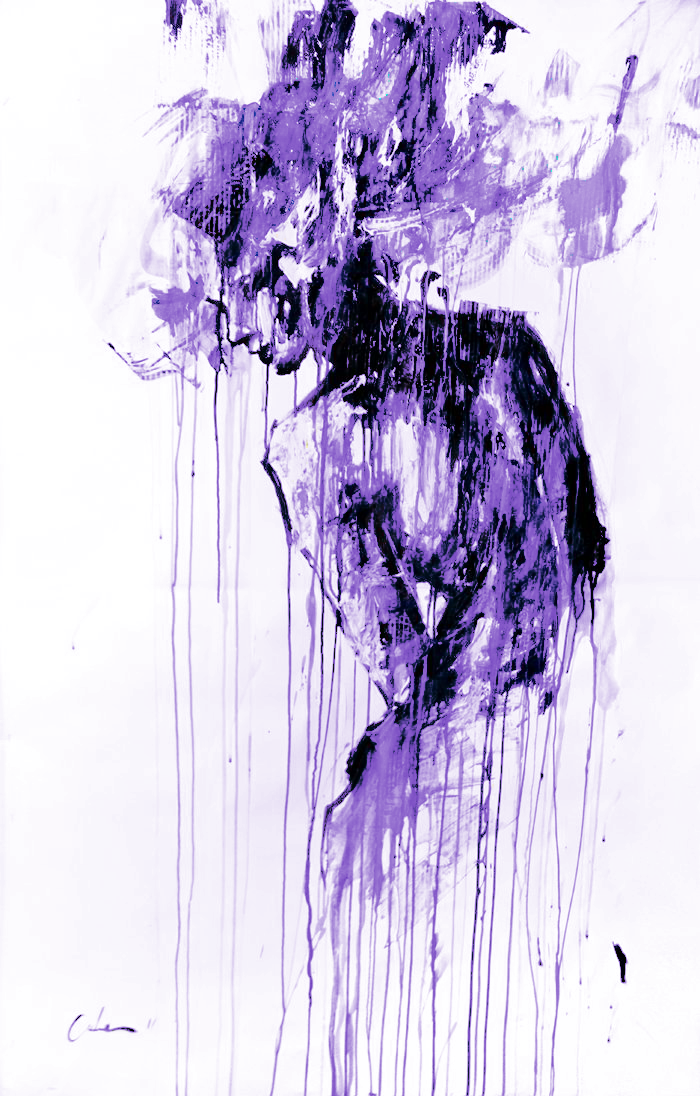
\includegraphics[width=\paperwidth]{pictures/decor/girl2}}; % Background image
\draw[anchor=north] (midpoint) node [fill=prpl!30!white,fill opacity=0.6,text opacity=1,inner sep=0.8cm]{\Huge\centering\bfseries\sffamily\parbox[c][][t]{\paperwidth}{\centering { \textcolor{black!100}{\fontsize{24.88}{14}\selectfont GOS-Book}}\\[4pt] % Book title
%{\Large }\\[20pt] % Subtitle
{\textcolor{black!100}{\huge Didenko Andr\'e}}\\[2pt] % Author name
{\textcolor{black!100}{\LARGE Edition from \twodigit\day.\twodigit\month.\the\year}}
}}; 
\end{tikzpicture}};
\end{tikzpicture}
\vfill

\newpage
\thispagestyle{empty}
\epigraph{Умереть не страшно, страшно не жить.}{Виктор Гюго}\centering
\vspace*{-0.7\baselineskip}  
\settowidth{\unitlength}{\LARGE\scshape Московский Физико"--~Технический Институт}
\begin{figure}[!h]
\center
\includegraphics[width=0.18\textwidth]{pictures/MIPT2}
\vspace{-0.5\baselineskip}
\end{figure}
{\LARGE\scshape Московский Физико"--~Технический Институт}
{\large \itshape Sapere aude}\\[0.14\baselineskip]
\rule{\unitlength}{1.7pt}\vspace*{-\baselineskip}\vspace*{2pt}
\rule{\unitlength}{0.4pt}\\[0.6\baselineskip]
{\Huge Подготовка к ГОСу по Матану}\\[0.4\baselineskip]
\rule{\unitlength}{0.4pt}\vspace*{-1.5\baselineskip}\vspace{3.2pt}
\rule{\unitlength}{1.7pt}\\[0.55\baselineskip]
{\large\scshape Диденко Андрей \\\vspace*{0.1\baselineskip}  %\normalsize студент 311 группы
}\par
\vspace*{0.35\baselineskip}  

{\LARGE\scshape Редакция от \twodigit\day.\twodigit\month.\the\year \;(\currenttime)}\par 

\vspace*{-1\baselineskip}  
\begin{flushleft}
\section*{\Large Полезные ссылки}
\begin{itemize}[wide, labelwidth=!, labelindent=0pt, label=$\blacktriangleright$, noitemsep]
\item Последняя версия книги в pdf-формате:

\qquad\href{https://GOS-Book.github.io/GOS-Book.pdf}{$
\begin{array}{l}
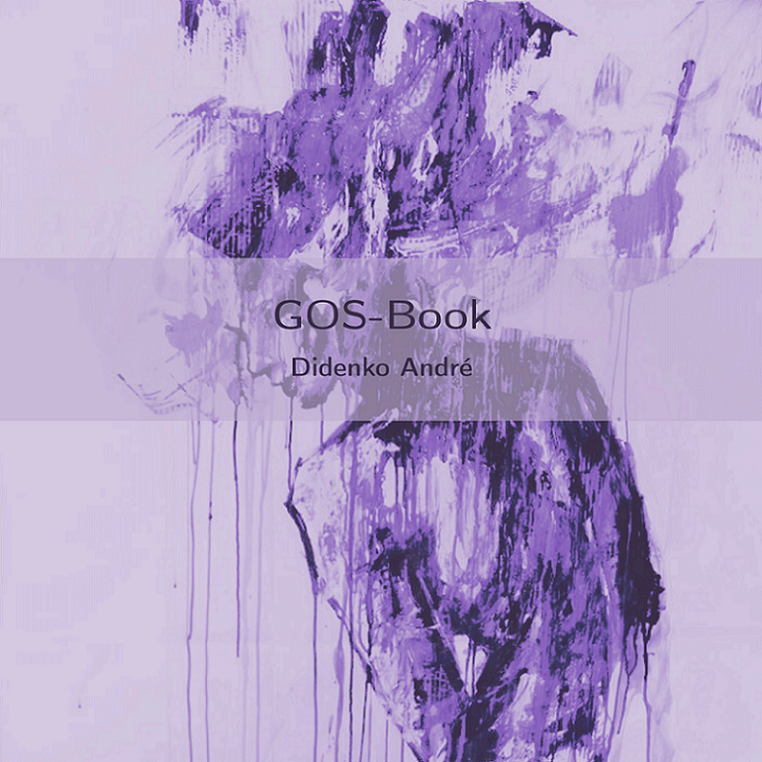
\includegraphics[width=\iconwidth]{pictures/reference/GitORG}
\end{array}
$\large GOS-Book.github.io/GOS-Book.pdf}

\item Web-site, посвященный данной книге:

\qquad\href{https://GOS-Book.github.io/}{$
\begin{array}{l}
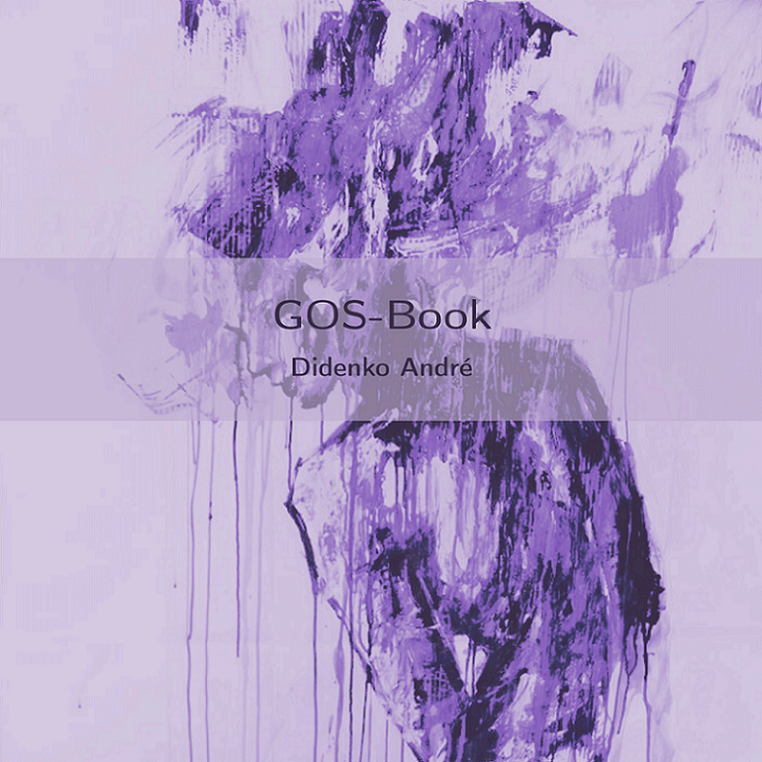
\includegraphics[width=\iconwidth]{pictures/reference/GitORG}
\end{array}
$\large GOS-Book.github.io}

\item Дополнительные материалы, полезные при подготовке как к \textit{устному} экзамену, так и к \textit{письменному} доступны по ссылке:

\qquad\href{https://drive.google.com/drive/u/0/folders/0BzuzEyNkpwYDYjVNcE0wa3hqWjA}{$
\begin{array}{l}

\includegraphics[width=\iconwidth]{pictures/reference/drive}
\end{array}
$\large drive.google.com/...}

\item Литература по курсам доступна по ссылке:

\qquad\href{https://drive.google.com/drive/u/0/folders/0BzuzEyNkpwYDcENXcV9jNWdwVlU}{$
\begin{array}{l}

\includegraphics[width=\iconwidth]{pictures/reference/drive}
\end{array}
$\large drive.google.com/...}

\item Анкета о ГОСе для ознакомления, также прошу вас заполнить ее после сдачи экзамена:

\qquad\href{https://docs.google.com/spreadsheets/d/1l2de9_qlCLvvqJIK8ZY6rtk_TJQbvo8cWd5o7uVtl2M/edit\#gid=0}{$
\begin{array}{l}

\includegraphics[width=\iconwidth]{pictures/reference/drive}
\end{array}
$\large drive.google.com/...}

\item Github-репозиторий, в котором хранится этот документ:

\qquad\href{https://github.com/GOS-Book/GOS-Book.github.io}{$
\begin{array}{l}

\includegraphics[width=\iconwidth]{pictures/reference/git}
\end{array}
$\large /GOS-Book/GOS-Book.github.io}

\item По любым вопросам касательно книги, также если вы хотите помочь в написании материала, просьба обращаться в личные сообщения: 

\qquad\href{https://t.me/didenko_andre}{$
	\begin{array}{l}
	
\includegraphics[width=\iconwidth]{pictures/reference/telegram}
	\end{array}
	$\large /didenko\_\!andre}
\qquad\href{https://vk.com/didenko_andre}{$
\begin{array}{l}

\includegraphics[width=\iconwidth]{pictures/reference/vk}
\end{array}
$\large /didenko\_\!andre}
\vspace*{-1\baselineskip}  
\end{itemize}

\section*{\Large Текущий статус книги}

$\blacktriangleright$ В данный момент потихоньку переписываю книгу к новой программе 2018 года и совершенствую остальной материал. Но срочно нужна помощь в написании и редактировании билетов. Поэтому если кто-то хочет помочь "--- прошу написать мне. 

\smallskip

\vfill

\textcolor{red}{
$\blacktriangleright$ Я крайне не рекомендую использовать данное пособие как \textit{\textbf{основную}} литературу во время подготовки к Государственному экзамену.
}

\end{flushleft}

\medskip
\vfill
{\huge\scshape I\;$\heartsuit$\;\LaTeX}\\[0.5\baselineskip]
{\LARGE\scshape 2016}\par
\restoregeometry
\endgroup
\newpage